\documentclass[11pt]{article}
% Shared preamble of the RMC kernel write-ups (% Shared preamble of the RMC kernel write-ups (% Shared preamble of the RMC kernel write-ups (\input{preamble} after \documentclass).
\usepackage[margin=1in]{geometry}
\usepackage{amsmath,amssymb,bm}
\usepackage{graphicx}
\usepackage{booktabs}
\usepackage{hyperref}

\newcommand{\dd}{\,\mathrm{d}}
\newcommand{\Ein}{E}
\newcommand{\Eout}{E'}
\newcommand{\Ecm}{E_{c}}
\newcommand{\mucm}{\mu_{c}}
\newcommand{\mulab}{\mu_0}

% Common closing section: how the verification figures are produced
\newcommand{\verificationmethod}{%
Each figure is produced by \texttt{verification/verify\_laws.py}. For an incident
energy $\Ein$ along $+z$, $10^6$ collisions are sampled with MC/DC's own reaction
sampler (\texttt{sample\_elastic\_scattering}, \texttt{sample\_inelastic\_scattering}
or \texttt{sample\_fission}), and every emitted neutron is histogrammed in
$48 \times 24$ bins of $(\Eout, \mulab)$, with $\mulab$ the lab cosine to $+z$. The
inverted kernel used by RMC is integrated over the same bins (Gauss--Legendre panels;
two-body lines are split where $\mulab^*(\Eout)$ crosses a cosine edge), multiplied by
the number of collisions, and compared with a $\chi^2$ test over bins with at least 5
expected counts (the rest pooled into one bin). The tables list $\chi^2/\mathrm{dof}$,
its $p$-value, the emitted neutrons per collision (sampled vs.\ the integral of the
inverted kernel), and the largest relative change of a bin integral when the
quadrature panels are doubled. Left panels: outgoing-energy marginal; middle:
lab-cosine marginal; right: per-bin $z = (\text{sampled} - \text{inverted}) /
\sqrt{\text{inverted}}$.}
 after \documentclass).
\usepackage[margin=1in]{geometry}
\usepackage{amsmath,amssymb,bm}
\usepackage{graphicx}
\usepackage{booktabs}
\usepackage{hyperref}

\newcommand{\dd}{\,\mathrm{d}}
\newcommand{\Ein}{E}
\newcommand{\Eout}{E'}
\newcommand{\Ecm}{E_{c}}
\newcommand{\mucm}{\mu_{c}}
\newcommand{\mulab}{\mu_0}

% Common closing section: how the verification figures are produced
\newcommand{\verificationmethod}{%
Each figure is produced by \texttt{verification/verify\_laws.py}. For an incident
energy $\Ein$ along $+z$, $10^6$ collisions are sampled with MC/DC's own reaction
sampler (\texttt{sample\_elastic\_scattering}, \texttt{sample\_inelastic\_scattering}
or \texttt{sample\_fission}), and every emitted neutron is histogrammed in
$48 \times 24$ bins of $(\Eout, \mulab)$, with $\mulab$ the lab cosine to $+z$. The
inverted kernel used by RMC is integrated over the same bins (Gauss--Legendre panels;
two-body lines are split where $\mulab^*(\Eout)$ crosses a cosine edge), multiplied by
the number of collisions, and compared with a $\chi^2$ test over bins with at least 5
expected counts (the rest pooled into one bin). The tables list $\chi^2/\mathrm{dof}$,
its $p$-value, the emitted neutrons per collision (sampled vs.\ the integral of the
inverted kernel), and the largest relative change of a bin integral when the
quadrature panels are doubled. Left panels: outgoing-energy marginal; middle:
lab-cosine marginal; right: per-bin $z = (\text{sampled} - \text{inverted}) /
\sqrt{\text{inverted}}$.}
 after \documentclass).
\usepackage[margin=1in]{geometry}
\usepackage{amsmath,amssymb,bm}
\usepackage{graphicx}
\usepackage{booktabs}
\usepackage{hyperref}

\newcommand{\dd}{\,\mathrm{d}}
\newcommand{\Ein}{E}
\newcommand{\Eout}{E'}
\newcommand{\Ecm}{E_{c}}
\newcommand{\mucm}{\mu_{c}}
\newcommand{\mulab}{\mu_0}

% Common closing section: how the verification figures are produced
\newcommand{\verificationmethod}{%
Each figure is produced by \texttt{verification/verify\_laws.py}. For an incident
energy $\Ein$ along $+z$, $10^6$ collisions are sampled with MC/DC's own reaction
sampler (\texttt{sample\_elastic\_scattering}, \texttt{sample\_inelastic\_scattering}
or \texttt{sample\_fission}), and every emitted neutron is histogrammed in
$48 \times 24$ bins of $(\Eout, \mulab)$, with $\mulab$ the lab cosine to $+z$. The
inverted kernel used by RMC is integrated over the same bins (Gauss--Legendre panels;
two-body lines are split where $\mulab^*(\Eout)$ crosses a cosine edge), multiplied by
the number of collisions, and compared with a $\chi^2$ test over bins with at least 5
expected counts (the rest pooled into one bin). The tables list $\chi^2/\mathrm{dof}$,
its $p$-value, the emitted neutrons per collision (sampled vs.\ the integral of the
inverted kernel), and the largest relative change of a bin integral when the
quadrature panels are doubled. Left panels: outgoing-energy marginal; middle:
lab-cosine marginal; right: per-bin $z = (\text{sampled} - \text{inverted}) /
\sqrt{\text{inverted}}$.}


\title{Inverted kernel: reactions with several spectra and an energy-dependent yield}
\date{}

\begin{document}
\maketitle

\noindent Code: \texttt{\_spectrum\_weight}, \texttt{\_secondaries\_through},
\texttt{continuous\_lab\_density} in \texttt{mcdc/rmc/reaction.py}.

\section{What MC/DC samples}

\texttt{sample\_inelastic\_scattering} for a reaction with $N_s$ energy spectra
(probabilities $p_n(\Ein)$ tabulated on a grid, histogram in $\Ein$) and multiplicity
$N$:
\begin{itemize}
  \item integer multiplicity: $N$ fixed; tabulated yield $\nu(\Ein)$ (ACE
  $|TY| > 100$): $N = \lfloor \nu(\Ein) + \xi\rfloor$;
  \item if $N = N_s$, secondary $n$ uses spectrum $n$ (each spectrum exactly once);
  \item otherwise every secondary picks spectrum $n$ with probability $p_n(\Ein)$.
\end{itemize}

\section{Expected emission per spectrum}

The kernel needs the expected number of neutrons emitted through spectrum $n$. For a
given $N$,
\begin{equation}
  s_n(N) = \begin{cases} 1 & N = N_s,\\ N\,p_n(\Ein) & \text{otherwise}.\end{cases}
\end{equation}
With $m = \lfloor\nu\rfloor$ and $\phi = \nu - m$, $N = m$ with probability $1 - \phi$
and $m+1$ with probability $\phi$, so
\begin{equation}
  w_n(\Ein) = (1-\phi)\,s_n(m) + \phi\,s_n(m+1),
\end{equation}
and for an integer multiplicity simply $w_n = s_n(N)$. Since $\sum_n s_n(N) = N$ in
both cases, $\sum_n w_n = \mathbb{E}[N] = \nu$. The reaction kernel is
\begin{equation}
  f_L(\Eout, \mulab \mid \Ein) = \sum_{n=1}^{N_s} w_n(\Ein)\,
  f_{L,n}(\Eout, \mulab \mid \Ein),
\end{equation}
with $f_{L,n}$ the per-neutron lab density of spectrum $n$ (and the reaction's angular
law). Note the rule at $N = N_s$: with a non-integer yield the mixture weights are not
simply $\nu p_n$. This replaces RMC's earlier rejection of multi-spectrum reactions
with a tabulated yield.

\paragraph{Data.} No reaction in the 293.6\,K library combines several spectra with a
tabulated yield, so the verification uses Li-7 MT-16 with a second spectrum (the data's
table compressed to half the outgoing energies), probabilities $0.3/0.7$, and
$\nu = 1.6$: $N \in \{1, 2\}$, and when $N = 2 = N_s$ each spectrum is used once.

\section{Verification}
\verificationmethod

\begin{center}
\begin{tabular}{rrrrrrr}
\toprule
$E$ [eV] & samples & bins & $\chi^2/\mathrm{dof}$ & $p$ & yield (sampled / inverted) & quad. err. \\
\midrule
1.2e+07 & 1e+06 & 1117 & 1075.8/1117 & 0.807 & 1.60041 / 1.60000 & 2.1e-05 \\
\bottomrule
\end{tabular}

\end{center}

\begin{figure}[h]
  \centering
  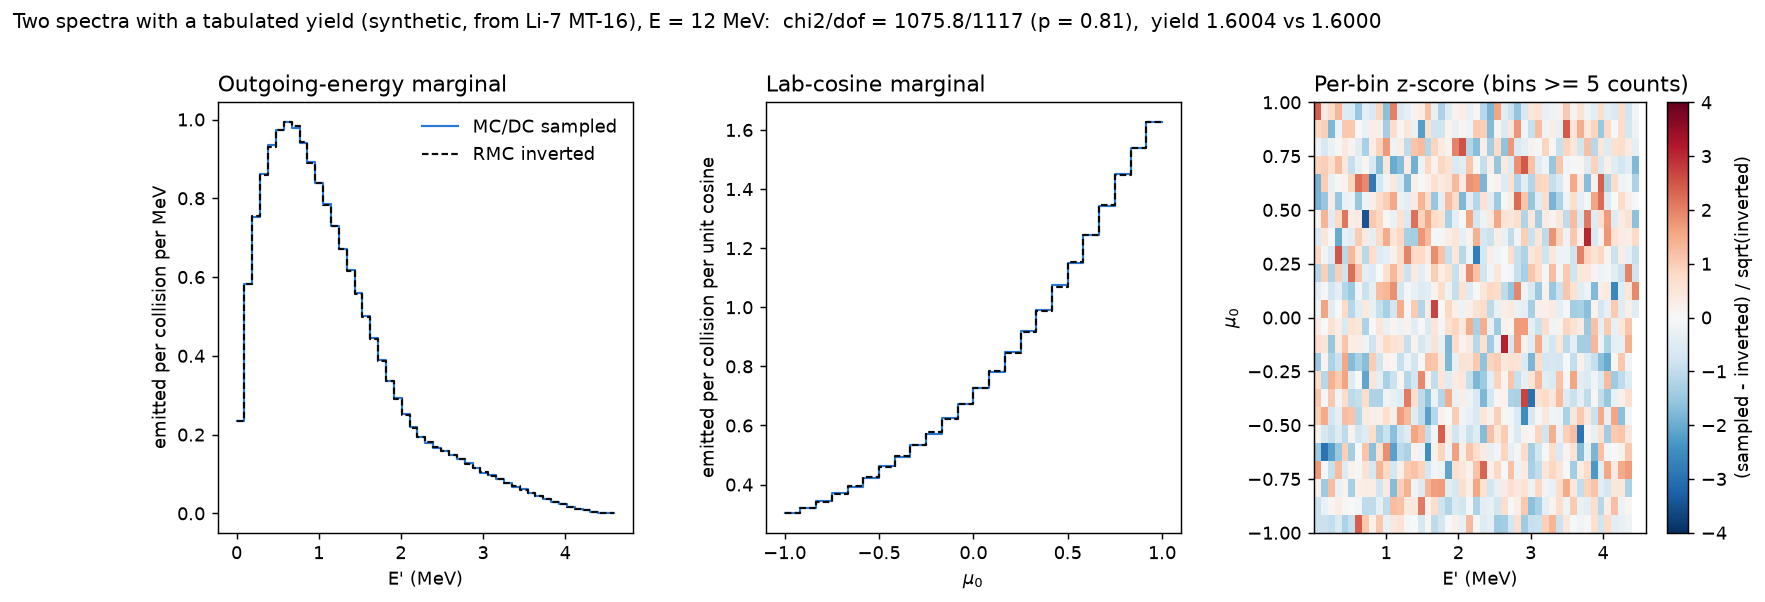
\includegraphics[width=\textwidth]{figures/multi_spectrum_yield/multi_spectrum_yield_E1p2e07.png}
  \caption{Synthetic two-spectrum reaction with $\nu = 1.6$ at 12\,MeV. The yield
  column checks $\sum_n w_n = \nu$ against the sampled neutrons per collision.}
\end{figure}

\end{document}
